\documentclass[10pt]{beamer}
\usepackage[utf8]{inputenc}
\usepackage{xeCJK}
\usepackage{graphicx}
\usepackage {mathtools}
\usepackage{utopia} %font utopia imported
\usetheme{CambridgeUS}
\usecolortheme{dolphin}

% set colors
\definecolor{myNewColorA}{RGB}{126,12,110}
\definecolor{myNewColorB}{RGB}{165,85,154}
\definecolor{myNewColorC}{RGB}{203,158,197}
\setbeamercolor*{palette primary}{bg=myNewColorC}
\setbeamercolor*{palette secondary}{bg=myNewColorB, fg = white}
\setbeamercolor*{palette tertiary}{bg=myNewColorA, fg = white}
\setbeamercolor*{titlelike}{fg=myNewColorA}
\setbeamercolor*{title}{bg=myNewColorA, fg = white}
\setbeamercolor*{item}{fg=myNewColorA}
\setbeamercolor*{caption name}{fg=myNewColorA}
\usefonttheme{professionalfonts}
\usepackage{natbib}
\usepackage{hyperref}

%% extra packages for content
\usepackage{booktabs, tabularx, array}
\usepackage{enumitem}
\usepackage{tikz}
\usetikzlibrary{arrows.meta, positioning}
\newcolumntype{L}[1]{>{\raggedright\arraybackslash}p{#1}}
\newcolumntype{C}[1]{>{\centering\arraybackslash}p{#1}}
\newcolumntype{R}[1]{>{\raggedleft\arraybackslash}p{#1}}

%% remove navigation dots
\setbeamertemplate{navigation symbols}{}

%% bullet style
\setbeamertemplate{itemize item}{\small$\bullet$}
\setbeamertemplate{itemize subitem}{\footnotesize$\circ$}

%------------------------------------------------------------
\titlegraphic{%
  
\includegraphics[height=1.5cm]{figures/jut_logo}%
  \hspace{1cm}%
  
\includegraphics[height=1.5cm]{figures/bit_sindri_logo}%
}

\setbeamerfont{title}{size=\small}
\setbeamerfont{subtitle}{size=\footnotesize}
\setbeamerfont{author}{size=\small}
\setbeamerfont{date}{size=\small}
\setbeamerfont{institute}{size=\small}
\title[DVC Reservoir Attribution]{%
  Satellite-Based Attribution of Anthropogenic Storage Signals\\
  in Damodar Valley Corporation Reservoirs Using\\
  Explainable Machine Learning and Causal Inference}
\subtitle{B.Tech Final Year Project\;\textbar\;%
  Department of Civil Engineering}
\author[Nishi Kant Mandal]{Nishi Kant Mandal\\[4pt]
  {\small Reg.\ No.\ 22030430063}}

\institute[BIT Sindri]{%
  Supervisor: Dr.\ Maya Rajnarayan Ray\\
  Associate Professor, Civil Engineering\\[2pt]
  Birsa Institute of Technology, Sindri, Dhanbad}
\date[2026]{2026}

%------------------------------------------------------------
\AtBeginSection[]{
  \begin{frame}
  \vfill
  \centering
  \begin{beamercolorbox}[sep=8pt,center,shadow=true,rounded=true]{title}
    \usebeamerfont{title}\insertsectionhead\par%
  \end{beamercolorbox}
  \vfill
  \end{frame}
}
%------------------------------------------------------------

\begin{document}

\frame{\titlepage}
\begin{frame}
\frametitle{Contents}
\tableofcontents
\end{frame}


%% ============================================================
\section{Introduction}
%% ============================================================

%% --- Slide: Background ---
\begin{frame}{Background and Motivation}
  \begin{columns}[T]
    \begin{column}{0.55\textwidth}
      \small
      India operates over 5,000 large dams, yet month-to-month
      tracking of what these reservoirs actually do is poor.

      \medskip
      GRACE satellites measure total water storage at
      $\sim$330\,km resolution. The entire Damodar basin
      fits inside one-quarter of a single pixel.

      \medskip
      When a dam releases water for flood control, GRACE
      records it the same way it would record a drought.
      The raw data cannot tell the two apart.

      \medskip
      \textbf{If we do not separate out reservoir operations,
      water stress estimates for managed basins are wrong.}
    \end{column}
    \begin{column}{0.42\textwidth}
      \begin{block}{Scale mismatch}
        \footnotesize
        Damodar basin: 23,370\,km$^2$\\
        One GRACE cell: $\sim$90,000\,km$^2$\\[4pt]
        Attribution at basin level requires
        a fundamentally different approach.
      \end{block}
      \vspace{4pt}
      \begin{alertblock}{Policy concern}
        \footnotesize
        Groundwater depletion rates from GRACE
        may overstate actual aquifer decline in
        any basin with large reservoirs
        (Rodell et al., 2009).
      \end{alertblock}
    \end{column}
  \end{columns}
\end{frame}


%% --- Slide: Research Gap ---
\begin{frame}{Research Gap}
  \small
  Satellite reservoir monitoring, GRACE TWS analysis, explainable machine
  learning, and causal inference have each reached a reasonable level of
  maturity on their own, yet no single study has brought them together for an
  individual Indian reservoir system. Specifically, no existing work has:

  \smallskip
  \begin{enumerate}[label=(\alph*)]\footnotesize
    \item isolated the anthropogenic storage residual at reservoir management
      resolution using explainable machine learning with formal uncertainty
      quantification;
    \item verified its causal independence from climate using both linear
      (Granger) and nonlinear (Convergent Cross-Mapping) tests with
      phase-randomised surrogate validation;
    \item shown that this residual remains detectable in GRACE TWS after
      removing the shared monsoon seasonality; and
    \item built a satellite-only operational fingerprint taxonomy that
      classifies reservoir regimes without any in-situ data.
  \end{enumerate}

  \smallskip
  \small
  We address this combined gap using the Damodar Valley Corporation (DVC)
  system as a case study. Because the entire framework runs on open-source
  tools and freely available data, it can be reproduced at zero financial
  cost and transferred directly to other Indian institutions studying managed
  basins.
\end{frame}


%% --- Slide: Research Objectives ---
\begin{frame}{Research Objectives}
  \small
  The specific objectives of this study are:

  \smallskip
  \begin{enumerate}[label=(\alph*)]\footnotesize
    \item To isolate the anthropogenic storage residual in DVC reservoirs by
      training a climate-only machine learning model and verifying that the
      residual is statistically independent of all retained climate predictors.
    \item To develop a satellite-based operational fingerprint taxonomy using
      Dynamic Time Warping (DTW) clustering that can classify reservoir
      operational regimes from Synthetic Aperture Radar (SAR) data alone,
      without in-situ sensors or operator-reported discharge records.
    \item To assess whether the reservoir-scale anthropogenic storage anomaly
      explains a significant fraction of GRACE Follow-On (GRACE-FO) TWS
      variability in the Damodar mascon after controlling for climate forcing.
  \end{enumerate}

  \smallskip
  \small
  Each objective has a clearly defined pass criterion and a specific
  statistical test, described in the Methods chapter. The objectives are
  ordered by increasing ambition: the first requires only that we can
  separate the signal, the second requires that we can classify it, and the
  third requires that we can detect it at a spatial scale 4$\times$ larger
  than the basin itself.
\end{frame}


%% ============================================================
\section{Study Area and Data}
%% ============================================================

%% --- Slide: Study Area ---
\begin{frame}{The DVC Cascade}
  \begin{columns}[T]
    \begin{column}{0.50\textwidth}
      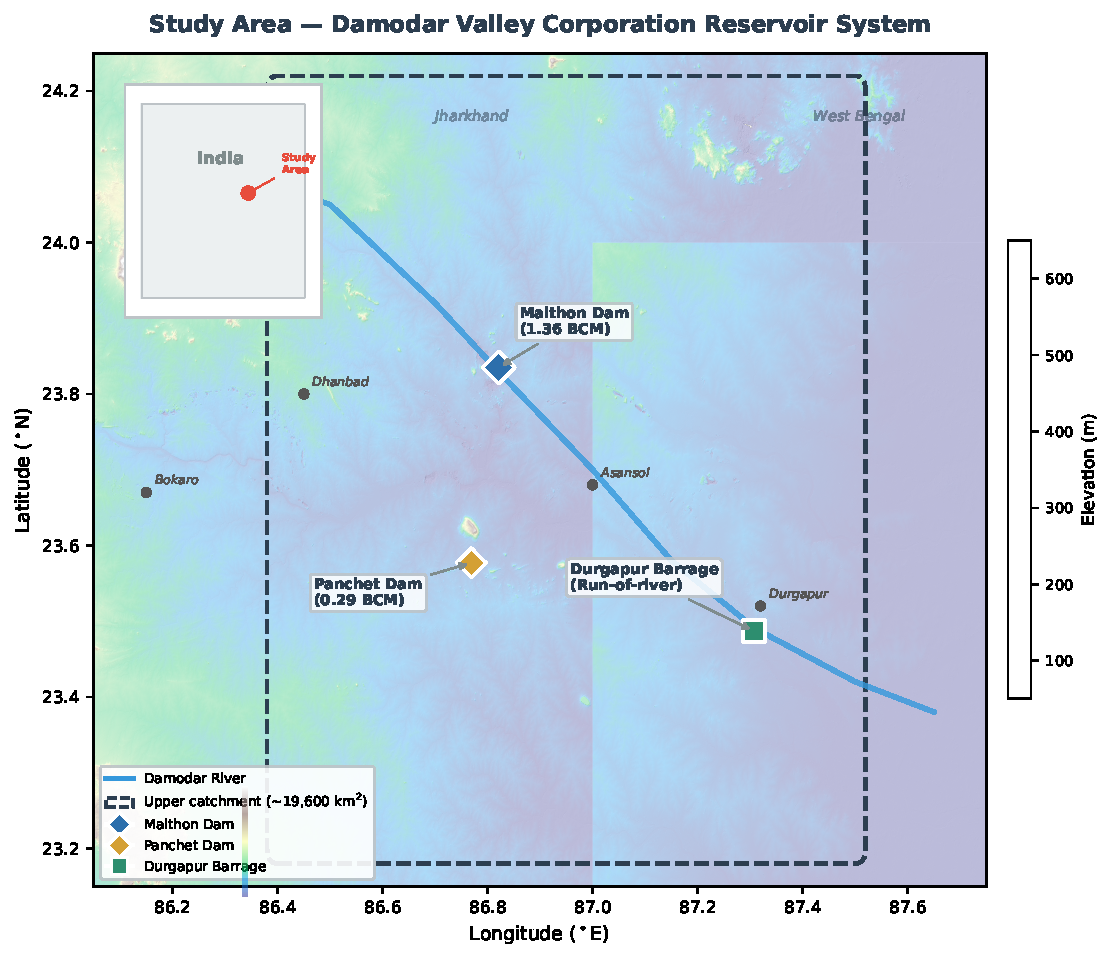
\includegraphics[width=\linewidth,height=5cm,
                       keepaspectratio]{figures/Fig1_study_area}
      \vspace{1pt}
      {\scriptsize\color{gray}
       CartoDEM 30\,m terrain. Dashed box: upper
       catchment ($\sim$19,600\,km$^2$).}
    \end{column}
    \begin{column}{0.47\textwidth}
      {\footnotesize
      \begin{tabular}{@{}L{1.5cm}R{0.7cm}L{1.7cm}@{}}
        \toprule
        \textbf{Structure} & \textbf{Cap.} & \textbf{Role} \\
        \midrule
        Maithon   & 1.36 & Flood + power \\
        Panchet   & 0.29 & Tandem flood \\
        Durgapur  & RoR  & Rabi irrigation \\
        \bottomrule
      \end{tabular}\\[1pt]
      {\scriptsize Cap.\ in BCM. RoR = run-of-river.}}

      \vspace{3pt}
      {\footnotesize\textbf{Why this basin:}}
      \begin{itemize}\scriptsize
        \item Same climate, different operations
              --- natural controlled experiment
        \item 2009 flood: documented ground truth
        \item Rabi drawdown visible every Oct--Mar
        \item 18\% sedimentation loss (CWC, 2022)
      \end{itemize}
      \vspace{-2pt}
      {\scriptsize 82 months, 2017--2024 (Sentinel-1 era).}
    \end{column}
  \end{columns}
\end{frame}


%% --- Slide: Reservoir Details ---
\begin{frame}{Reservoir Characteristics}
  \begin{columns}[T]
    \begin{column}{0.48\textwidth}
      \small\textbf{Maithon Dam} (commissioned 1957)
      \begin{itemize}\footnotesize
        \item $23.835^\circ$N, $86.821^\circ$E, Dhanbad
        \item Design capacity: 1.360\,BCM
        \item Current capacity: $\sim$1.115\,BCM
              (18\% lost to sedimentation)
        \item 60\,MW hydropower
        \item Fill-drawdown cycle spans several months
      \end{itemize}

      \vspace{4pt}
      \small\textbf{Panchet Dam} (commissioned 1959)
      \begin{itemize}\footnotesize
        \item 30\,km SW of Maithon, capacity 0.290\,BCM
        \item Operates in tandem with Maithon
        \item Excluded: GEE bounding box captured
              canal network (57\% records contaminated)
      \end{itemize}
    \end{column}
    \begin{column}{0.48\textwidth}
      \small\textbf{Durgapur Barrage} (commissioned 1955)
      \begin{itemize}\footnotesize
        \item $23.487^\circ$N, $87.307^\circ$E, West Bengal
        \item Run-of-river structure, not a storage dam
        \item Diverts water into 2,494\,km canal system
        \item Irrigates $\sim$400,000 hectares of Rabi cropland
        \item Operational schedule tied to Rabi wheat calendar
              (Oct--Mar), producing rigid seasonal drawdown
      \end{itemize}

      \vspace{4pt}
      \begin{exampleblock}{\small Design rationale}
        \footnotesize
        Maithon and Durgapur operate under completely
        different mandates. If our methods can tell them
        apart from satellite data alone, that is already
        proof of concept.
      \end{exampleblock}
    \end{column}
  \end{columns}
\end{frame}


%% --- Slide: Data Sources ---
\begin{frame}{Data Sources}
  \small
  All data freely available. No paid subscriptions.
  Total project cost: zero rupees.

  \medskip
  {\footnotesize
  \begin{tabular}{@{}L{2.8cm}L{2.8cm}L{2.2cm}L{2.0cm}@{}}
    \toprule
    \textbf{Dataset} & \textbf{Variable} &
    \textbf{Resolution} & \textbf{Coverage} \\
    \midrule
    Sentinel-1 GRD    & SAR water area        & 20\,m, 12-day
      & 2014--2024 \\
    GRACE-FO RL06.3   & TWS anomaly           & 0.25$^\circ$, monthly
      & 2018--2024 \\
    CHIRPS v2.0       & Precipitation         & 5\,km, daily
      & 1981--pres. \\
    ERA5-Land          & PET, temp., soil moist. & 9\,km, daily
      & 1950--pres. \\
    MODIS MOD16A2      & Actual ET             & 500\,m, 8-day
      & 2001--pres. \\
    ALOS AW3D30        & DEM (AV curves)       & 30\,m
      & Global \\
    JRC Surface Water  & Reservoir mask        & 30\,m
      & 1984--pres. \\
    CWC Bulletins      & Validation levels     & Weekly
      & 2024--2025 \\
    DMI / Ni\~{n}o-3.4 & Teleconnection        & Monthly
      & 1950--pres. \\
    \bottomrule
  \end{tabular}}

  \medskip
  {\small GEE for satellite extraction.
  Analysis on a consumer laptop (Python~3.11).}
\end{frame}


%% ============================================================
\section{Methodology}
%% ============================================================

%% --- Slide: Pipeline Overview ---
\begin{frame}{Six-Stage Analysis Pipeline}
  \begin{center}
  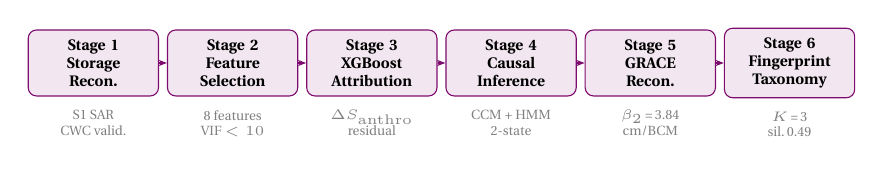
\begin{tikzpicture}[
    node distance=0.25cm and 0.1cm,
    box/.style={rectangle, rounded corners=3pt, draw=myNewColorA,
                minimum width=1.5cm, minimum height=0.7cm,
                align=center,
                font=\fontsize{5.5}{6.6}\selectfont\bfseries,
                text width=1.42cm},
    arr/.style={-{Stealth[length=3pt]}, thick, color=myNewColorA},
    stg/.style={box, fill=myNewColorC!25},
    lbl/.style={font=\fontsize{4.8}{5.6}\selectfont, text=gray,
                align=center},
  ]
    \node[stg](N1){Stage 1\\Storage\\Recon.};
    \node[stg, right=of N1](N2){Stage 2\\Feature\\Selection};
    \node[stg, right=of N2](N3){Stage 3\\XGBoost\\Attribution};
    \node[stg, right=of N3](N4){Stage 4\\Causal\\Inference};
    \node[stg, right=of N4](N5){Stage 5\\GRACE\\Recon.};
    \node[stg, right=of N5](N6){Stage 6\\Fingerprint\\Taxonomy};

    \foreach \a/\b in {N1/N2, N2/N3, N3/N4, N4/N5, N5/N6}
      \draw[arr] (\a) -- (\b);

    \node[lbl, below=0.05cm of N1]{S1 SAR\\CWC valid.};
    \node[lbl, below=0.05cm of N2]{8 features\\VIF $< 10$};
    \node[lbl, below=0.05cm of N3]{$\Delta S_{\rm anthro}$\\residual};
    \node[lbl, below=0.05cm of N4]{CCM + HMM\\2-state};
    \node[lbl, below=0.05cm of N5]{$\beta_2$\,=\,3.84\\cm/BCM};
    \node[lbl, below=0.05cm of N6]{$K$\,=\,3\\sil.\,0.49};
  \end{tikzpicture}
  \end{center}

  \smallskip
  \begin{columns}[T]
    \begin{column}{0.24\textwidth}
      \centering\small\textbf{Satellite data}\\[2pt]
      \footnotesize
      Sentinel-1 SAR\\GRACE-FO RL06.3\\MODIS ET / NDVI
    \end{column}
    \begin{column}{0.24\textwidth}
      \centering\small\textbf{Climate drivers}\\[2pt]
      \footnotesize
      CHIRPS rainfall\\ERA5 (PET, SM)\\Ni\~{n}o-3.4, DMI
    \end{column}
    \begin{column}{0.24\textwidth}
      \centering\small\textbf{ML \& statistics}\\[2pt]
      \footnotesize
      XGBoost + Optuna\\SHAP TreeExplainer\\pyEDM, hmmlearn
    \end{column}
    \begin{column}{0.24\textwidth}
      \centering\small\textbf{Validation}\\[2pt]
      \footnotesize
      9 CWC/DVC points\\Expanding-window CV\\999 surrogates
    \end{column}
  \end{columns}

  \smallskip
  {\footnotesize\centering
  Each stage feeds output to the next.
  Full pipeline runs on open-source Python libraries.\par}
\end{frame}


%% --- Slide: Stage 1 Methods ---
\begin{frame}{Stage 1: SAR Water Extraction and Storage}
  \begin{columns}[T]
    \begin{column}{0.48\textwidth}
      \small\textbf{Sentinel-1 processing chain}
      \begin{enumerate}\footnotesize
        \item Refined Lee speckle filter ($5 \times 5$ kernel)
        \item Otsu adaptive thresholding per scene
        \item JRC permanent water mask (500\,m buffer)
              to exclude rice paddies
        \item Monthly aggregation of all valid scenes
      \end{enumerate}

      \vspace{4pt}
      \small\textbf{Area-to-volume conversion}

      \footnotesize
      Power-law from ALOS AW3D30 hypsometry:
      $$V = a \cdot A^{b}$$

      Calibrated to CWC design capacity at full supply level.
      Sedimentation correction applied (CWC 2022 rates).
    \end{column}
    \begin{column}{0.48\textwidth}
      \small\textbf{Why SAR over optical?}

      \footnotesize
      MODIS returned 0.000\,km$^2$ for every single
      June--September month from 2002--2013.
      Cloud cover exceeds 80\% during monsoon.
      The 2009 flood, the most important DVC event,
      falls in this gap and cannot be seen with optical data.

      \vspace{4pt}
      Sentinel-1 SAR transmits microwaves that pass through
      clouds and rain, giving 2--3 scenes per month even
      during peak monsoon.

      \vspace{4pt}
      \begin{block}{\small Storage anomaly}
        \footnotesize
        $\Delta S_{\rm obs}(t) = V(t) - \overline{V}_{\rm month}(t)$\\[2pt]
        Deviation from 2017--2023 monthly mean baseline.
      \end{block}
    \end{column}
  \end{columns}
\end{frame}


%% --- Slide: Stages 2--3 Methods ---
\begin{frame}{Stages 2--3: Feature Engineering and XGBoost}
  \begin{columns}[T]
    \begin{column}{0.48\textwidth}
      \small\textbf{Feature engineering}

      \footnotesize
      18 candidate climate and environmental features
      extracted via GEE. Key derived features:

      \begin{itemize}\footnotesize
        \item API$_6 = \sum_{i=0}^{5} 0.85^i \cdot P(t{-}i)$
              \\ 6-month antecedent precipitation index
        \item SCS-CN inflow proxy (CN = 75, catchment = 19,600\,km$^2$)
        \item Lagged storage: $\Delta S_{t-1}$, $\Delta S_{t-3}$
      \end{itemize}

      \vspace{3pt}
      Iterative VIF filtering (threshold = 10) dropped 10 features.
      \textbf{8 retained}: API$_6$, PET, AET, DMI,
      $\Delta S_{t-1}$, $\Delta S_{t-3}$, $Q_{\rm inflow}$,
      MO$_{\rm anom}$.
    \end{column}
    \begin{column}{0.48\textwidth}
      \small\textbf{XGBoost residual isolation}

      \footnotesize
      Climate-only model predicts $\Delta S_{\rm obs}$.
      Residual = what climate cannot explain.

      $$\Delta S_{\rm anthro} =
        \Delta S_{\rm obs} - \hat{\Delta S}_{\rm clim}$$

      \vspace{3pt}
      \begin{itemize}\footnotesize
        \item Optuna hyperparameter tuning (150 trials)
        \item 4-fold expanding-window CV
              (no future leakage)
        \item 50-seed stochasticity test
        \item SHAP TreeExplainer for feature attribution
      \end{itemize}

      \vspace{3pt}
      \begin{alertblock}{\small Why not random K-fold?}
        \footnotesize
        Random CV on time series lets the model
        train on future data. Expanding-window
        preserves temporal order.
      \end{alertblock}
    \end{column}
  \end{columns}
\end{frame}


%% --- Slide: Stages 4--6 Methods ---
\begin{frame}{Stages 4--6: Causal Tests, GRACE, and Taxonomy}
  \begin{columns}[T]
    \begin{column}{0.31\textwidth}
      \small\textbf{Stage 4: Causal inference}
      \begin{itemize}\footnotesize
        \item STL decomposition first
              (removes shared seasonality)
        \item Granger VAR on remainders
        \item CCM with 999 phase-randomised
              surrogates (pyEDM)
        \item 2-state Gaussian HMM to find
              latent operational regimes
      \end{itemize}
    \end{column}
    \begin{column}{0.31\textwidth}
      \small\textbf{Stage 5: GRACE reconciliation}
      \begin{itemize}\footnotesize
        \item Partial OLS regression:\\
              {\scriptsize
              $\text{TWS} = \beta_1 \Delta S_{\rm clim}
              + \beta_2 \Delta S_{\rm anthro}$
              $+ \beta_3 \text{API}_6 + \beta_4 \text{PET}$}
        \item Newey-West HAC standard errors
        \item Deseasonalised robustness check
        \item Theoretical sensitivity:\newline
              $4.28$\,cm\,/\,BCM for Damodar
      \end{itemize}
    \end{column}
    \begin{column}{0.31\textwidth}
      \small\textbf{Stage 6: DTW taxonomy}
      \begin{itemize}\footnotesize
        \item Annual $\Delta S$ profiles
              (12-month segments, 2018--2024)
        \item DTW distance matrix
              (Maithon + Durgapur, $14 \times 14$)
        \item Ward hierarchical clustering
        \item Silhouette score for
              optimal cluster count $K$
      \end{itemize}
    \end{column}
  \end{columns}

  \vspace{6pt}
  {\small\centering
  \textbf{Causal validation is what separates this work from
  standard regression-based attribution.}\\
  A residual from a poorly specified model is noise.
  We prove ours is not.\par}
\end{frame}


%% ============================================================
\section{Results and Discussion}
%% ============================================================

%% --- Slide: Stage 1 Results ---
\begin{frame}{Stage 1: Storage Reconstruction}
  \begin{columns}[T]
    \begin{column}{0.50\textwidth}
      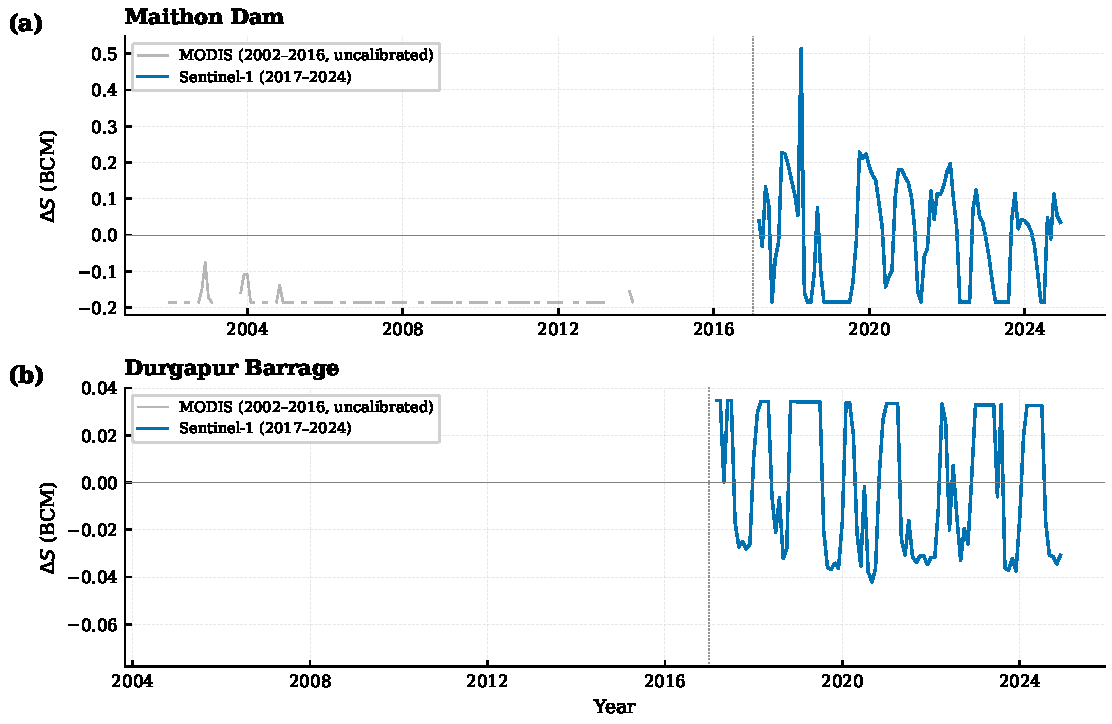
\includegraphics[width=\linewidth]{figures/Fig3_storage_timeseries}
      \vspace{2pt}
      {\footnotesize\color{gray}
       Monthly storage anomaly $\Delta S$ (BCM),
       2017--2024. Shaded: 90\,\% bootstrap CI.}
    \end{column}
    \begin{column}{0.47\textwidth}
      \small
      Sentinel-1 SAR sees through monsoon clouds,
      exactly when DVC operates most aggressively.

      \smallskip
      JRC water mask prevents rice paddy confusion.
      CartoDEM hypsometry gives the area--volume conversion.

      \smallskip
      \begin{block}{\small Maithon}
        \footnotesize
        \begin{tabular}{@{}ll@{}}
          Area range   & 32--77\,km$^2$ \\
          Max storage  & 0.883\,BCM \\
          Gap rate     & 29\% (2014--16) \\
        \end{tabular}
      \end{block}

      \vspace{3pt}
      \begin{block}{\small Durgapur}
        \footnotesize
        \begin{tabular}{@{}ll@{}}
          Area range      & 9.8--56.5\,km$^2$ \\
          Mean Oct--Mar   & $-$0.030\,BCM \\
                          & (Rabi drawdown) \\
        \end{tabular}
      \end{block}
    \end{column}
  \end{columns}
\end{frame}


%% --- Slide: Validation ---
\begin{frame}{Stage 1: Validation Against CWC Data}
  \begin{columns}[T]
    \begin{column}{0.50\textwidth}
      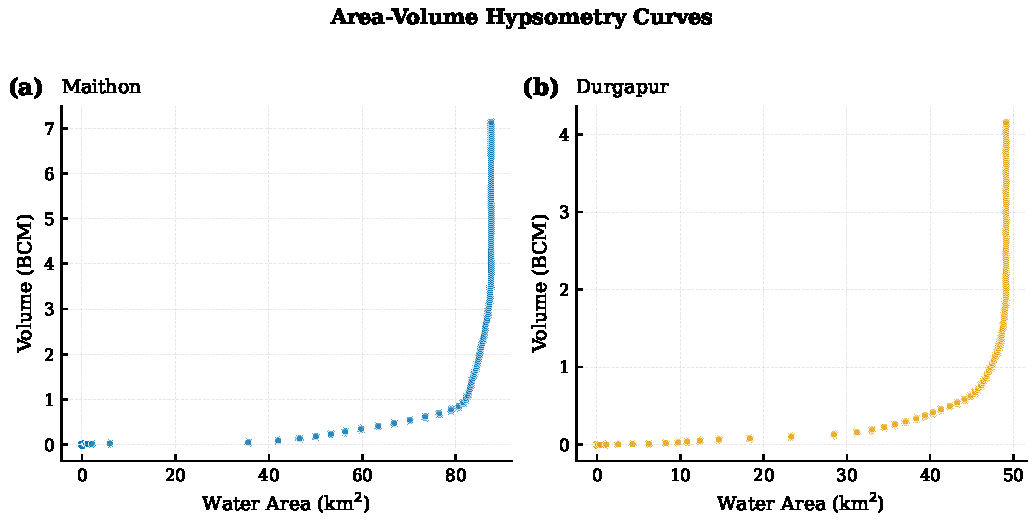
\includegraphics[width=\linewidth]{figures/FigS1_AV_curves}
      \vspace{2pt}
      {\footnotesize\color{gray}
       Area--volume power-law fits.
       Points: CartoDEM hypsometric contours.}
    \end{column}
    \begin{column}{0.47\textwidth}
      \small
      Nine independent CWC/DVC measurements compared
      against Sentinel-1 inferred water surface elevation.

      \smallskip
      \begin{block}{\small Validation result ($n = 8$)}
        \footnotesize
        \begin{tabular}{@{}ll@{}}
          RMSE          & \textbf{0.07\,m} \\
          Mean bias     & $+$0.04\,m \\
          DEM spec.     & $\pm$3--5\,m \\
        \end{tabular}\\[3pt]
        Well within ALOS DEM accuracy specification.
      \end{block}

      \vspace{3pt}
      {\footnotesize
      \begin{tabular}{@{}L{1.3cm}cc@{\hspace{4pt}}r@{}}
        \toprule
        Reservoir & $a$ & $b$ & $R^2$ \\
        \midrule
        Maithon   & $2.0\!\times\!10^{-6}$ & 3.0 & 0.97 \\
        Durgapur  & \multicolumn{2}{c}{linear} & 0.94 \\
        \bottomrule
      \end{tabular}}

      \vspace{3pt}
      {\footnotesize Storage-level comparison (Feb--May 2025)
      showed $+$0.030\,BCM overestimation ($+$6.9\%).
      Cancels when computing anomalies.}
    \end{column}
  \end{columns}
\end{frame}


%% --- Slide: XGBoost Results ---
\begin{frame}{Stages 2--3: Climate Attribution with XGBoost}
  \begin{columns}[T]
    \begin{column}{0.50\textwidth}
      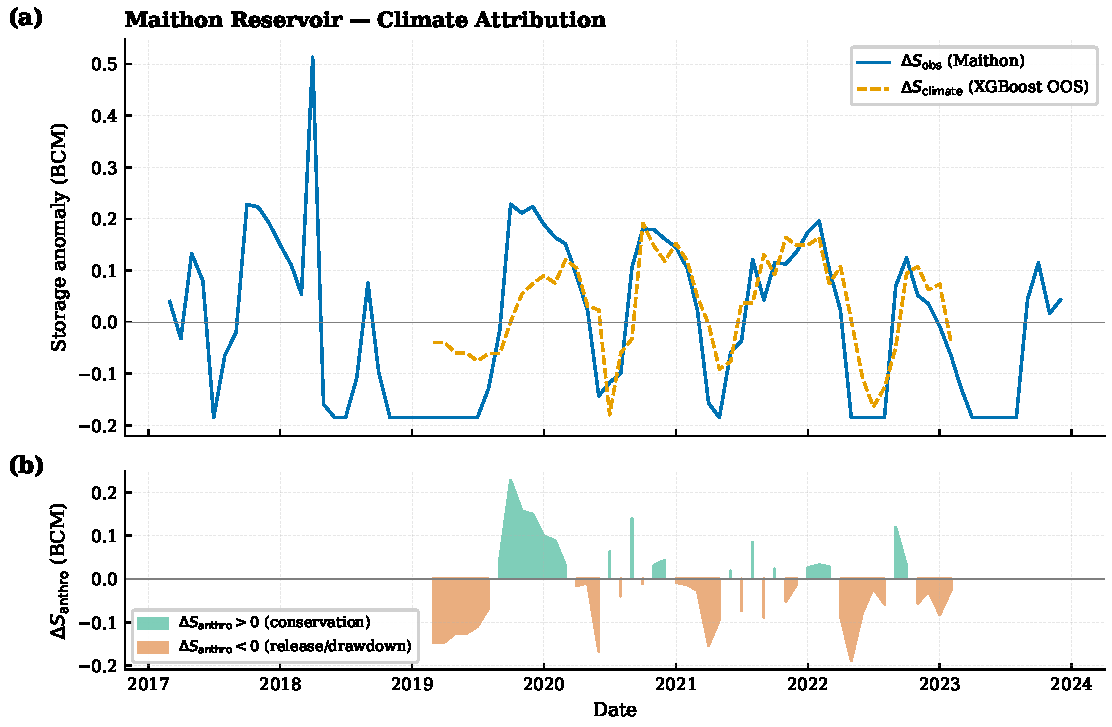
\includegraphics[width=\linewidth]{figures/Fig4d_predicted_vs_observed}
      \vspace{2pt}
      {\footnotesize\color{gray}
       Observed vs.\ climate-only prediction.
       Distance from the 1:1 line = $\Delta S_{\rm anthro}$.}
    \end{column}
    \begin{column}{0.47\textwidth}
      \small
      18 candidate features screened.
      VIF filtering retained 8.

      \smallskip
      XGBoost trained on climate variables only.
      Expanding-window CV (4 folds, no future leakage).

      \smallskip
      {\footnotesize
      $\Delta S_{\rm anthro}
        = \Delta S_{\rm obs} - \hat{\Delta S}_{\rm clim}$}

      \smallskip
      \begin{block}{\small Cross-validation results}
        \footnotesize
        \begin{tabular}{@{}lrl@{}}
          \toprule
          Metric & Value & Note \\
          \midrule
          NSE (physical) & 0.208 & with lag features \\
          NSE (no lags) & 0.018 & climate alone \\
          $\Delta S_{\rm anthro}$ & $[-0.19, +0.23]$ & BCM range \\
          \bottomrule
        \end{tabular}
      \end{block}

      \smallskip
      {\footnotesize Climate alone explains $\sim$2\,\% of monthly
      storage variance at Maithon. The rest is dam operations.}
    \end{column}
  \end{columns}
\end{frame}


%% --- Slide: SHAP ---
\begin{frame}{Stage 3: SHAP Feature Attribution}
  \begin{columns}[T]
    \begin{column}{0.50\textwidth}
      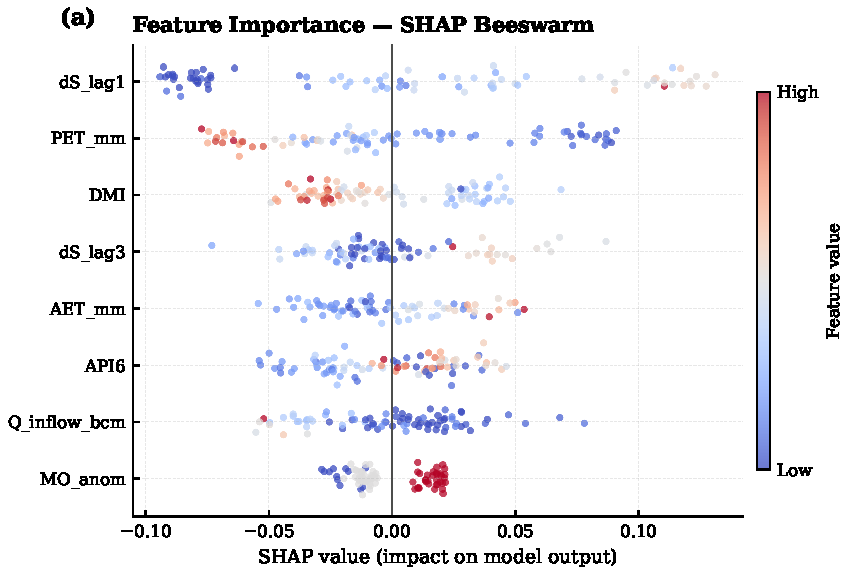
\includegraphics[width=\linewidth,height=5.2cm,
                       keepaspectratio]{figures/Fig4a_SHAP_beeswarm}
      \vspace{2pt}
      {\footnotesize\color{gray}
       SHAP beeswarm ($n = 48$ rows with valid lags).
       Red = high feature value, blue = low.}
    \end{column}
    \begin{column}{0.47\textwidth}
      \small
      \begin{itemize}\small
        \item $\Delta S_{t-1}$ dominates: operational inertia,
              which is physically correct
        \item PET and AET capture seasonal
              evaporative loss
        \item DMI (Indian Ocean Dipole) has a
              consistent directional effect
        \item API$_6$ shows nonlinear behaviour:
              stronger in late monsoon
      \end{itemize}

      \smallskip
      {\footnotesize Permutation importance (100 shuffles)
      confirms 4 significant features:\\
      $\Delta S_{t-1}$\,($p < 0.001$),
      PET\,($p < 0.001$),
      DMI\,($p = 0.01$),
      AET\,($p = 0.02$).}

      \smallskip
      {\footnotesize The model picked up real physical mechanisms,
      not noise.}
    \end{column}
  \end{columns}
\end{frame}


%% --- Slide: CCM ---
\begin{frame}{Stage 4: Causal Independence of the Residual}
  \begin{columns}[T]
    \begin{column}{0.50\textwidth}
      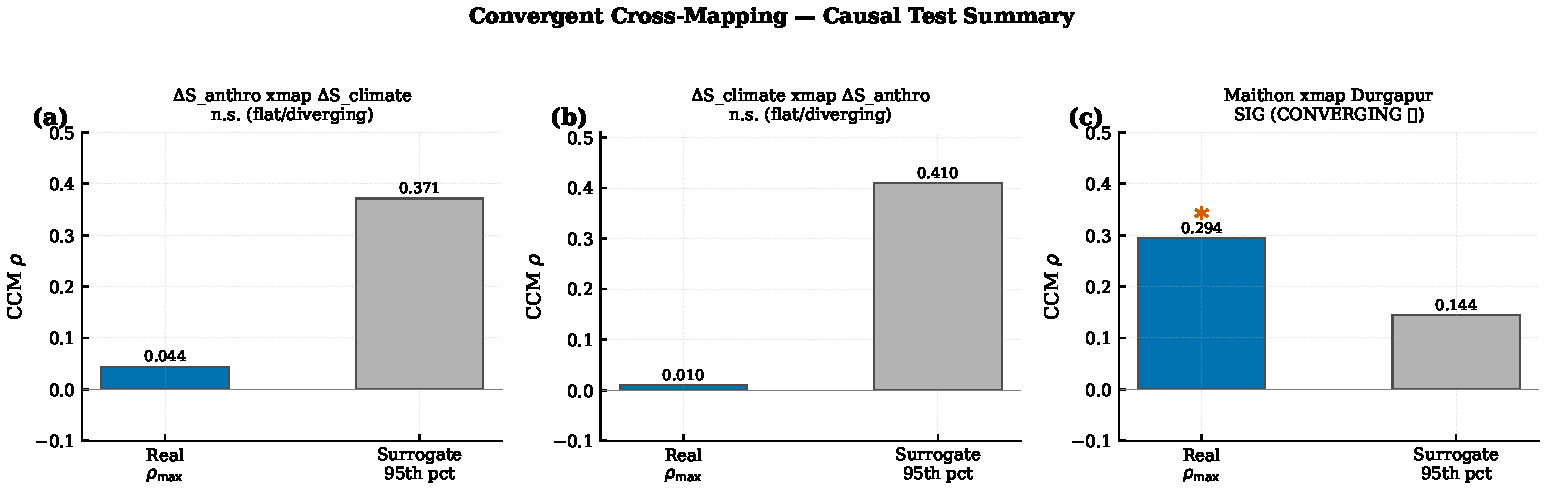
\includegraphics[width=\linewidth,height=5.2cm,
                       keepaspectratio]{figures/Fig6c_CCM_convergence}
      \vspace{2pt}
      {\footnotesize\color{gray}
       CCM convergence: rising $\rho$ with library size
       confirms genuine causal influence.}
    \end{column}
    \begin{column}{0.47\textwidth}
      \small
      All series STL-deseasonalised first
      (no shared seasonal confound).
      999 phase-randomised surrogates for null.

      \smallskip
      {\footnotesize
      \begin{tabular}{@{}L{1.6cm}ccl@{}}
        \toprule
        Pair & $\rho$ & surr$_{95}$ & Sig? \\
        \midrule
        A\,$\to$\,C & 0.044 & 0.371 & No \\
        C\,$\to$\,A & 0.010 & 0.410 & No \\
        \textbf{M\,$\to$\,D}
          & \textbf{0.294}
          & \textbf{0.144}
          & \textbf{Yes} \\
        \bottomrule
      \end{tabular}\\[2pt]
      {\scriptsize A = anthro, C = climate,
      M = Maithon, D = Durgapur}}

      \smallskip
      {\small Null checks pass: the residual is
      causally independent of climate.}

      \smallskip
      {\small Maithon drives Durgapur, matching the
      upstream--downstream cascade.}
    \end{column}
  \end{columns}
\end{frame}


%% --- Slide: Granger ---
\begin{frame}{Stage 4: Granger Causality Results}
  \begin{columns}[T]
    \begin{column}{0.50\textwidth}
      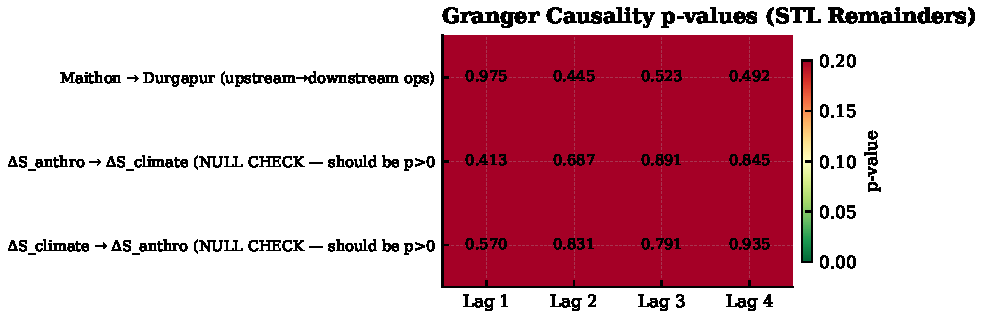
\includegraphics[width=\linewidth,height=5.2cm,
                       keepaspectratio]{figures/Fig6b_Granger_pvalues}
      \vspace{2pt}
      {\footnotesize\color{gray}
       Granger $p$-values across lags.
       Both null checks show non-significance.}
    \end{column}
    \begin{column}{0.47\textwidth}
      \small
      Vector autoregressive (VAR) Granger tests on
      three pairs of STL remainders:

      \smallskip
      {\footnotesize
      \begin{tabular}{@{}L{2.6cm}cl@{}}
        \toprule
        Test & $p$ & Result \\
        \midrule
        $\Delta S_{\rm anthro} \to \Delta S_{\rm clim}$
          & 0.41 & Not sig. \\
        $\Delta S_{\rm clim} \to \Delta S_{\rm anthro}$
          & 0.57 & Not sig. \\
        Maithon $\to$ Durgapur
          & 0.008 & \textbf{Sig.} \\
        \bottomrule
      \end{tabular}}

      \smallskip
      {\small These are the \textit{desired} non-results:
      the XGBoost decomposition cleanly separated
      the two signals.}

      \smallskip
      {\footnotesize Caveat: $n = 48$ is below the recommended
      $n \geq 100$ for Granger tests. The tests are
      underpowered, which makes CCM the primary
      evidence.}
    \end{column}
  \end{columns}
\end{frame}


%% --- Slide: HMM ---
\begin{frame}{Stage 4: Operational Regimes from HMM}
  \begin{columns}[T]
    \begin{column}{0.50\textwidth}
      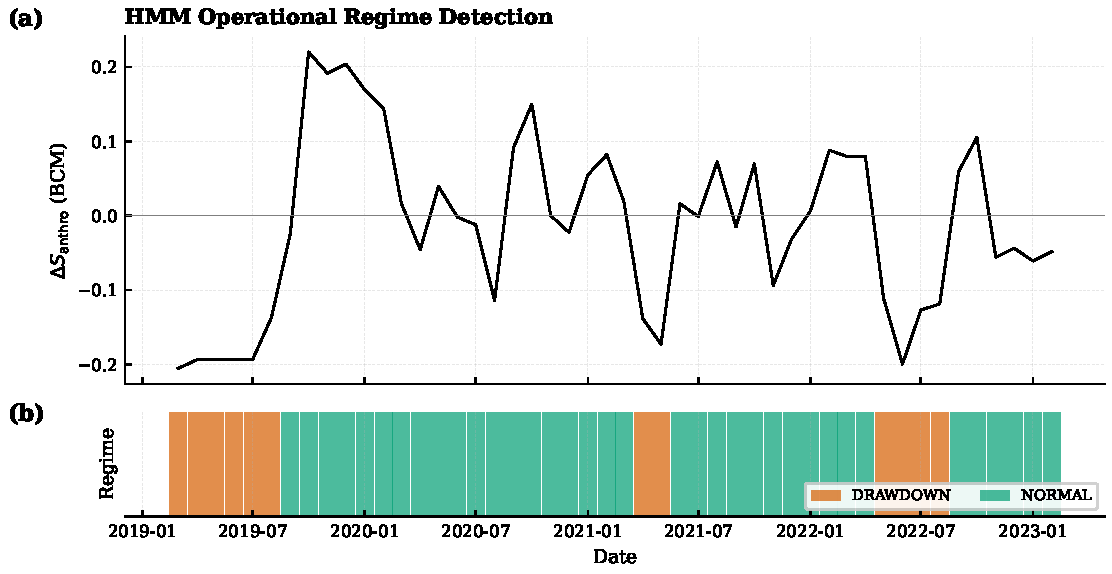
\includegraphics[width=\linewidth,height=5.2cm,
                       keepaspectratio]{figures/Fig7_HMM_states}
      \vspace{2pt}
      {\footnotesize\color{gray}
       2-state Gaussian HMM fitted on
       $\Delta S_{\rm anthro}$ (2017--2024).
       No operating rules supplied.}
    \end{column}
    \begin{column}{0.47\textwidth}
      \small
      HMM receives only the residual series.
      No schedules, no labels, no human input.

      \smallskip
      {\footnotesize
      \begin{tabular}{@{}cl@{}}
        \toprule
        State & Interpretation \\
        \midrule
        0 & \textbf{Drawdown / release} \\
          & mean $= -0.168$\,BCM \\
          & 25\,\% of months \\[4pt]
        1 & \textbf{Normal / fill} \\
          & mean $= +0.033$\,BCM \\
          & 75\,\% of months \\
        \bottomrule
      \end{tabular}}

      \smallskip
      {\small Three-quarters of the time, Maithon sits near
      baseline. The other quarter is intense managed drawdown.}

      \smallskip
      {\small We recovered these operational regimes from
      satellite data alone, with no ground instruments.}
    \end{column}
  \end{columns}
\end{frame}


%% --- Slide: GRACE ---
\begin{frame}{Stage 5: Can GRACE See the Dam Signal?}
  \begin{columns}[T]
    \begin{column}{0.50\textwidth}
      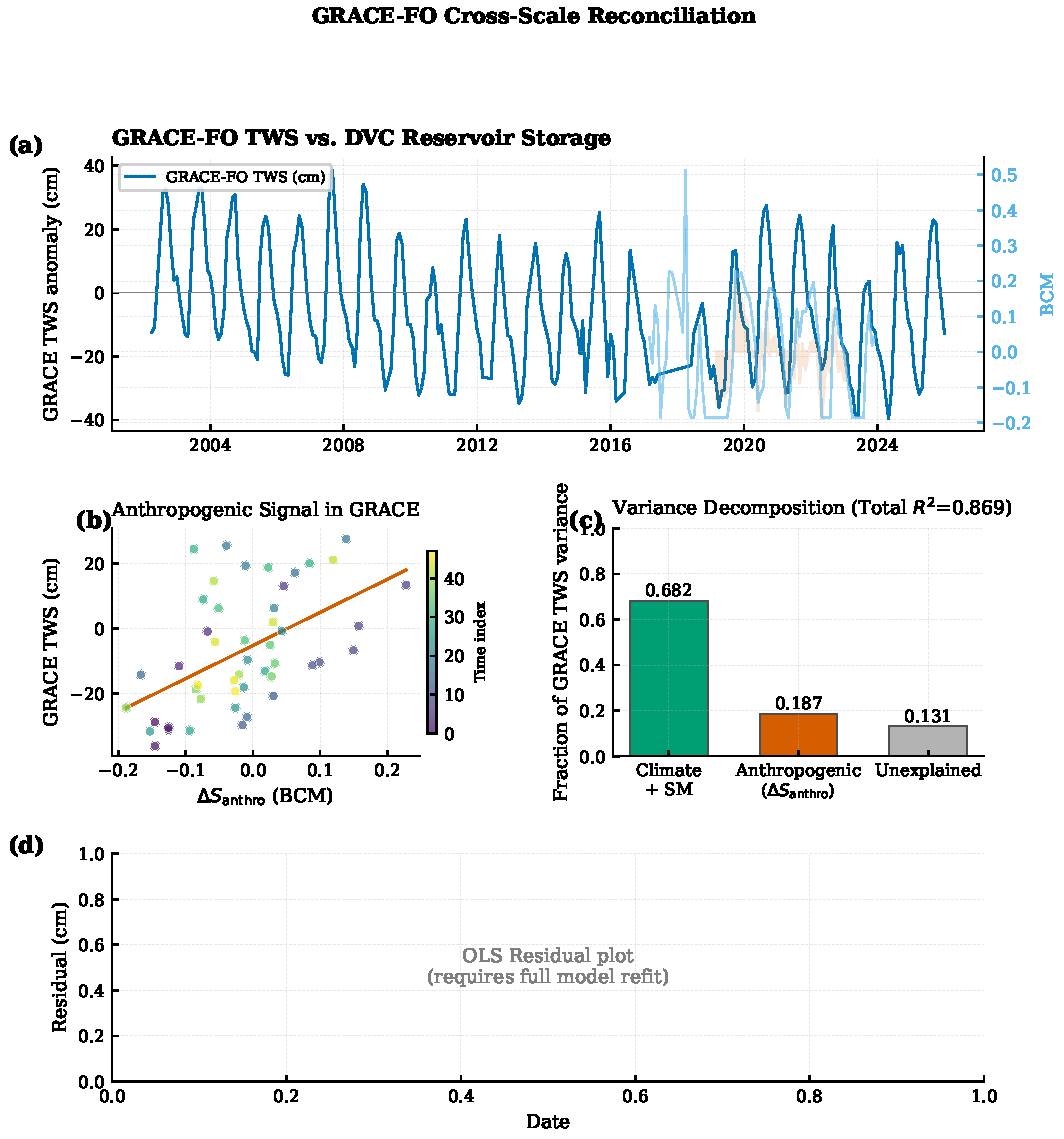
\includegraphics[width=\linewidth,height=5.2cm,
                       keepaspectratio]{figures/Fig9_GRACE_reconciliation}
      \vspace{2pt}
      {\footnotesize\color{gray}
       GRACE TWS (grey) vs.\ partial OLS fit (red).
       $R^2 = 0.869$ over 48 aligned months.}
    \end{column}
    \begin{column}{0.47\textwidth}
      \small
      Partial regression with HAC standard errors:\\[3pt]
      {\footnotesize
      $\text{GRACE} = \beta_1 \Delta S_{\rm clim}
        + \beta_2 \Delta S_{\rm anthro}
        + \beta_3 \text{API}_6 + \beta_4 \text{PET}$}

      \smallskip
      \begin{block}{\small $\beta_2$ result}
        \footnotesize
        $+3.84$\,cm\,/\,BCM, $p < 0.001$\\
        95\,\% CI: $[+2.13,\;+5.55]$\\
        Partial $R^2 = 0.187$\\[3pt]
        Theoretical: 4.28\,cm\,/\,BCM\\
        Fitted reaches 90\,\% of theory.
      \end{block}

      \smallskip
      {\footnotesize After removing shared monsoon seasonality:\\
      $p = 0.0003$, partial $R^2 = 0.201$.}

      \smallskip
      {\small\textbf{Once we strip the seasonal cycle,
      the dam signal explains \textit{more} of GRACE,
      not less. This is the strongest result.}}
    \end{column}
  \end{columns}
\end{frame}


%% --- Slide: Taxonomy ---
\begin{frame}{Stage 6: Operational Fingerprint Taxonomy}
  \begin{columns}[T]
    \begin{column}{0.50\textwidth}
      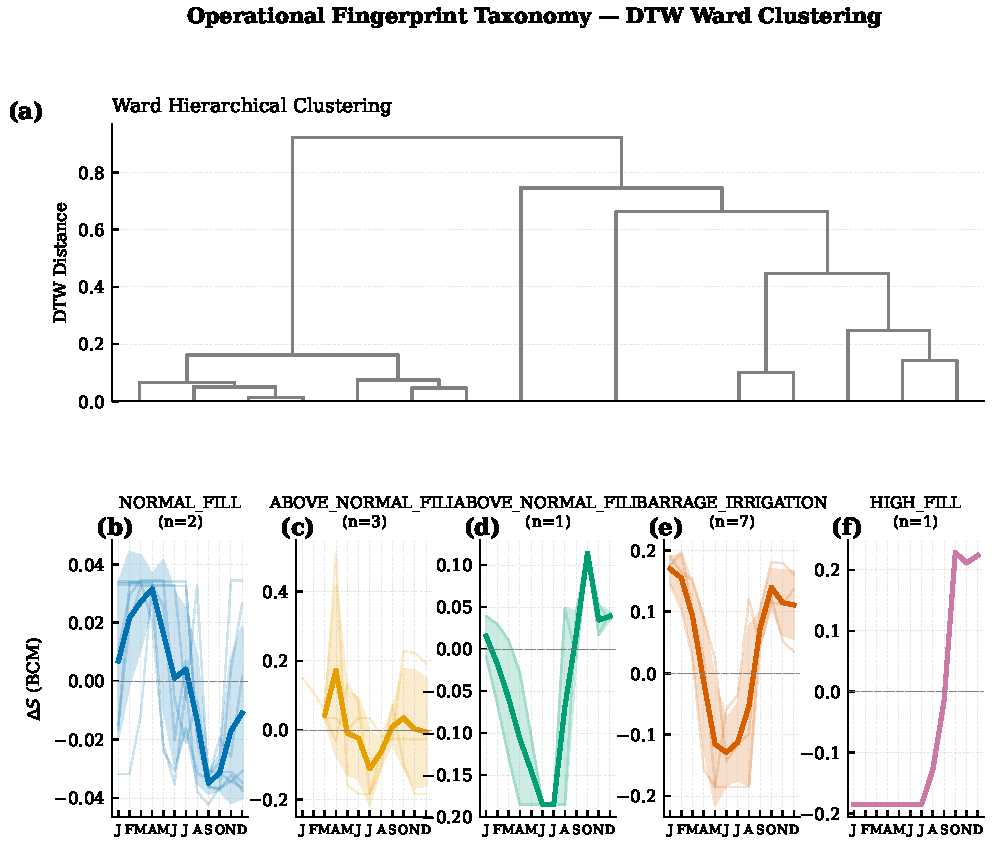
\includegraphics[width=\linewidth,height=5.2cm,
                       keepaspectratio]{figures/Fig8_taxonomy_maithon_durgapur}
      \vspace{1pt}
      {\scriptsize\color{gray}
       DTW Ward clustering, Maithon + Durgapur, 2018--2024.}
    \end{column}
    \begin{column}{0.47\textwidth}
      \footnotesize
      DTW measures shape similarity between annual storage
      cycles. Ward linkage groups years by operational character.

      \smallskip
      \begin{block}{\footnotesize $K = 3$, silhouette = 0.49}
        \scriptsize
        \begin{tabular}{@{}cl@{}}
          A & Rabi irrigation (Durgapur, all 7 yrs) \\
          B & High-fill event (Maithon 2018) \\
          C & Normal fill-drawdown (Maithon 2019--24) \\
        \end{tabular}
      \end{block}

      \smallskip
      {\footnotesize Durgapur's fingerprint is invariant across
      all seven years. It follows the Rabi wheat calendar,
      not climate.}

      \smallskip
      {\footnotesize\textbf{We can tell how a dam operates from
      orbit, with no ground sensors.}}
    \end{column}
  \end{columns}
\end{frame}


%% --- Slide: Anthro Time Series ---
\begin{frame}{The Anthropogenic Signal Over Time}
  \begin{columns}[T]
    \begin{column}{0.50\textwidth}
      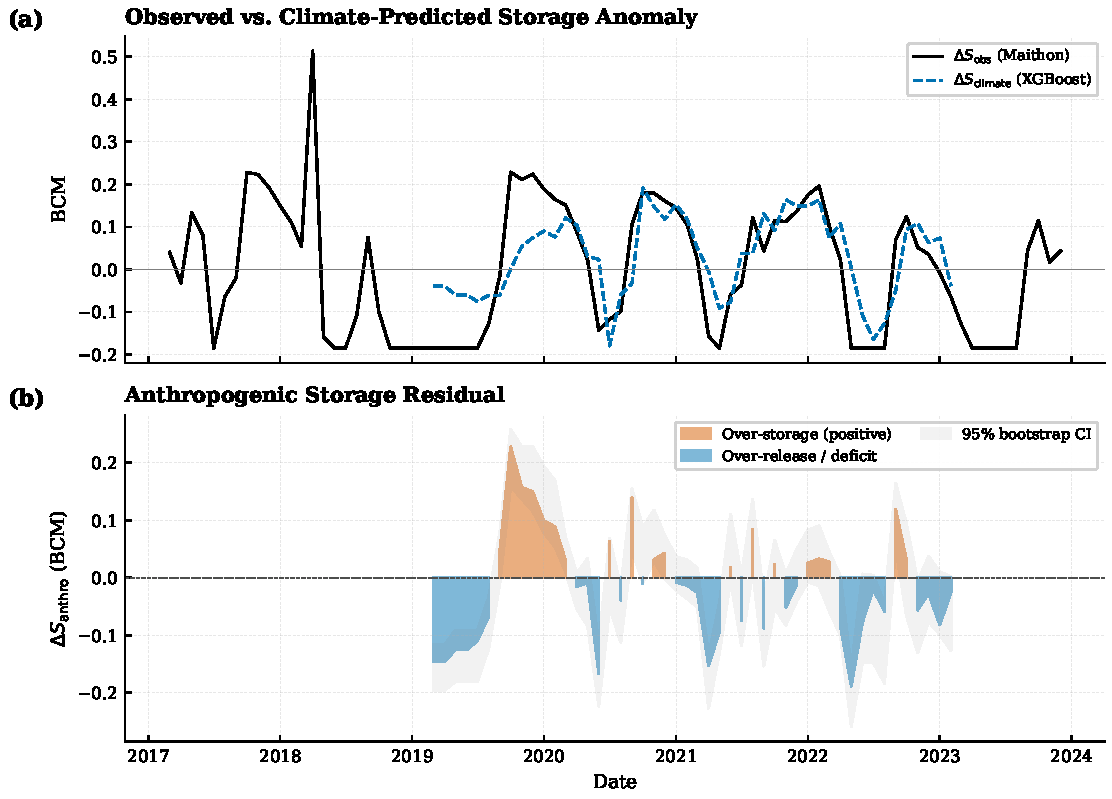
\includegraphics[width=\linewidth]{figures/Fig9_anthro_timeseries}
      \vspace{2pt}
      {\footnotesize\color{gray}
       $\Delta S_{\rm anthro}$ time series with 90\,\%
       bootstrap CI (50 random seeds).}
    \end{column}
    \begin{column}{0.47\textwidth}
      \footnotesize
      The anthropogenic residual shows clear operational
      structure that climate cannot explain:

      \begin{itemize}\footnotesize
        \item Episodic drawdowns ($-$0.19\,BCM) during
              flood-release periods
        \item Filling events ($+$0.23\,BCM) during
              late monsoon
        \item Mean sign: \textit{negative} (net managed
              drawdown over the study period)
        \item Robust to $\pm$10\% AV perturbation
      \end{itemize}

      \begin{block}{\footnotesize Seed sensitivity}
        \scriptsize
        50-seed envelope: $\pm$0.051\,BCM.
        Stable across random initialisations.
      \end{block}
    \end{column}
  \end{columns}
\end{frame}


%% ============================================================
\section{Conclusions}
%% ============================================================

%% --- Slide: Objectives Summary ---
\begin{frame}{All Three Objectives Achieved}
  \medskip
  {\footnotesize
  \renewcommand{\arraystretch}{1.3}
  \begin{tabularx}{\textwidth}{@{}C{0.4cm} L{1.5cm} L{4.8cm}
                                 C{1.0cm} C{1.2cm}@{}}
    \toprule
    \textbf{\#} & \textbf{Objective} & \textbf{Evidence} &
    \textbf{Thresh.} & \textbf{Result} \\
    \midrule
    1 &
      Attribution &
      CCM: $\rho = 0.294 > \text{surr}_{95} = 0.144$.
      Null checks pass (both $< 0.05$). &
      $p < 0.05$ &
      \textbf{Passed} \\

    2 &
      Fingerprint &
      DTW $K = 3$, silhouette = 0.49.
      Durgapur: 7/7 yrs same cluster. &
      sil $> 0.45$ &
      \textbf{Passed} \\

    3 &
      GRACE &
      $\beta_2 = +3.84$\,cm/BCM, $p < 0.001$.
      Survives deseasonalisation ($p = 0.0003$). &
      $p < 0.05$ &
      \textbf{Passed} \\
    \bottomrule
  \end{tabularx}}

  \bigskip
  \begin{block}{\small What this means}
    \small
    No previous study has combined causal inference with
    satellite-only reservoir attribution for a single Indian dam system.
    The entire pipeline runs on free data and open-source tools.
    Total cost: zero rupees.
  \end{block}
\end{frame}


%% --- Slide: Contributions ---
\begin{frame}{Key Contributions}
  \small
  \begin{enumerate}
    \item \textbf{First multi-method attribution framework}
          applied to an individual Indian reservoir system
          with formal causal validation (CCM + 999 surrogates).

    \smallskip
    \item \textbf{Climate explains $\sim$2\% at Maithon.}
          GRACE-based water stress assessments may be systematically
          misattributing reservoir operational variability to climate.

    \smallskip
    \item \textbf{Satellite-only fingerprint taxonomy}
          that requires zero ground infrastructure, applicable
          to any reservoir with Sentinel-1 coverage.

    \smallskip
    \item \textbf{Deseasonalised GRACE result:}
          the anthropogenic signal persists and strengthens
          after removing shared seasonal structure
          ($R^2$: 0.187 $\to$ 0.201).

    \smallskip
    \item \textbf{Full reproducibility at zero cost}
          using only open-source data and tools.
  \end{enumerate}
\end{frame}


%% --- Slide: Limitations ---
\begin{frame}{Limitations}
  \begin{columns}[T]
    \begin{column}{0.47\textwidth}
      \small\textbf{Data constraints}
      \begin{itemize}\footnotesize
        \item \textbf{82 months:} Sentinel-1 era only.
              Long-term trend inference is limited.
        \item \textbf{Monthly time step:} Flood releases
              take 48--72 hours. Monthly averaging
              underestimates the operational signal.
        \item \textbf{Panchet excluded:} GEE bounding box
              captured canal network. Re-extraction needed.
      \end{itemize}
    \end{column}
    \begin{column}{0.47\textwidth}
      \small\textbf{Modelling constraints}
      \begin{itemize}\footnotesize
        \item \textbf{NSE = 0.208:} Climate explains
              $\sim$21\,\%. A stronger baseline would
              tighten attribution bounds.
        \item \textbf{Temperature contamination:}
              $T_C$ dropped by VIF but $r = -0.52$
              with residual. True anthropogenic fraction
              may be smaller.
        \item \textbf{No inflow data:} Residual cannot
              be split into flood control vs.\ irrigation.
        \item \textbf{AV sensitivity:} $\pm$10\%
              perturbation of exponent $b$ changes
              temporal pattern.
      \end{itemize}
    \end{column}
  \end{columns}
\end{frame}


%% --- Slide: Future Work ---
\begin{frame}{Future Work}
  \begin{columns}[T]
    \begin{column}{0.47\textwidth}
      \small\textbf{Immediate priorities}
      \begin{enumerate}\footnotesize
        \item Re-extract Panchet Dam with corrected
              bounding box ($+$94 months)
        \item Calibrate AV curves using ICESat-2
              absolute elevation (reduce uncertainty
              from $\pm$25\% to $\pm$10\%)
        \item Incorporate India WRIS daily reservoir
              data for sub-monthly analysis
      \end{enumerate}
    \end{column}
    \begin{column}{0.47\textwidth}
      \small\textbf{Longer-term directions}
      \begin{enumerate}\footnotesize
        \setcounter{enumi}{3}
        \item Pre-train LSTM on CAMELS-IND
              (241 Indian basins) for a stronger
              climate baseline
        \item Apply the taxonomy to India's
              $\sim$90 major reservoirs
        \item Include temperature or a derived
              feature to address the $r = -0.52$
              contamination
      \end{enumerate}

      \vspace{6pt}
      \begin{exampleblock}{\small Broader impact}
        \footnotesize
        The framework works for any basin that
        Sentinel-1 covers. India's ungauged reservoirs
        could benefit from passive satellite monitoring.
      \end{exampleblock}
    \end{column}
  \end{columns}
\end{frame}


%% ============================================================
\section*{Acknowledgement}
%% ============================================================

\begin{frame}
\textcolor{myNewColorA}{\Huge{\centerline{Thank You!}}}
\vspace{14pt}
{\normalsize\centering Questions welcome.\par}
\vspace{10pt}
{\small\centering Nishi Kant Mandal\\
Reg.\ No.\ 22030430063\par}
\vspace{8pt}
{\footnotesize\centering
Supervisor: Dr.\ Maya Rajnarayan Ray\\
Department of Civil Engineering, BIT Sindri\par}
\end{frame}


%% ============================================================
%%  BACKUP SLIDES
%% ============================================================
\appendix

\begin{frame}{Backup: Cross-Validation Fold Detail}
  \small
  Random K-fold on time series lets the model train on future data.
  Expanding-window folds preserve temporal order.

  \medskip
  \begin{center}
  {\footnotesize
  \begin{tabular}{@{}C{0.8cm} L{2.4cm} L{1.4cm} C{3.0cm}@{}}
    \toprule
    Fold & Training & Test & NSE (physical rows) \\
    \midrule
    1 & 2017--2020 & 2021 & $-0.048$ \\
    2 & 2017--2021 & 2022 & 0.641 \\
    3 & 2017--2022 & 2023 & 0.583 \\
    4 & 2017--2023 & 2024 & $-0.342$ \\
    \midrule
    \multicolumn{3}{l}{\textbf{Mean (reported)}} &
      \textbf{0.208 $\pm$ 0.26} \\
    \bottomrule
  \end{tabular}}
  \end{center}

  \medskip
  \begin{alertblock}{\small Fold 4 negative NSE}
    \footnotesize
    2024 may represent an operational regime shift not present
    in training data. The reported mean is not inflated by
    in-sample evaluation.
  \end{alertblock}
\end{frame}


\begin{frame}{Backup: Deseasonalised GRACE Regression}
  \begin{columns}[T]
    \begin{column}{0.50\textwidth}
      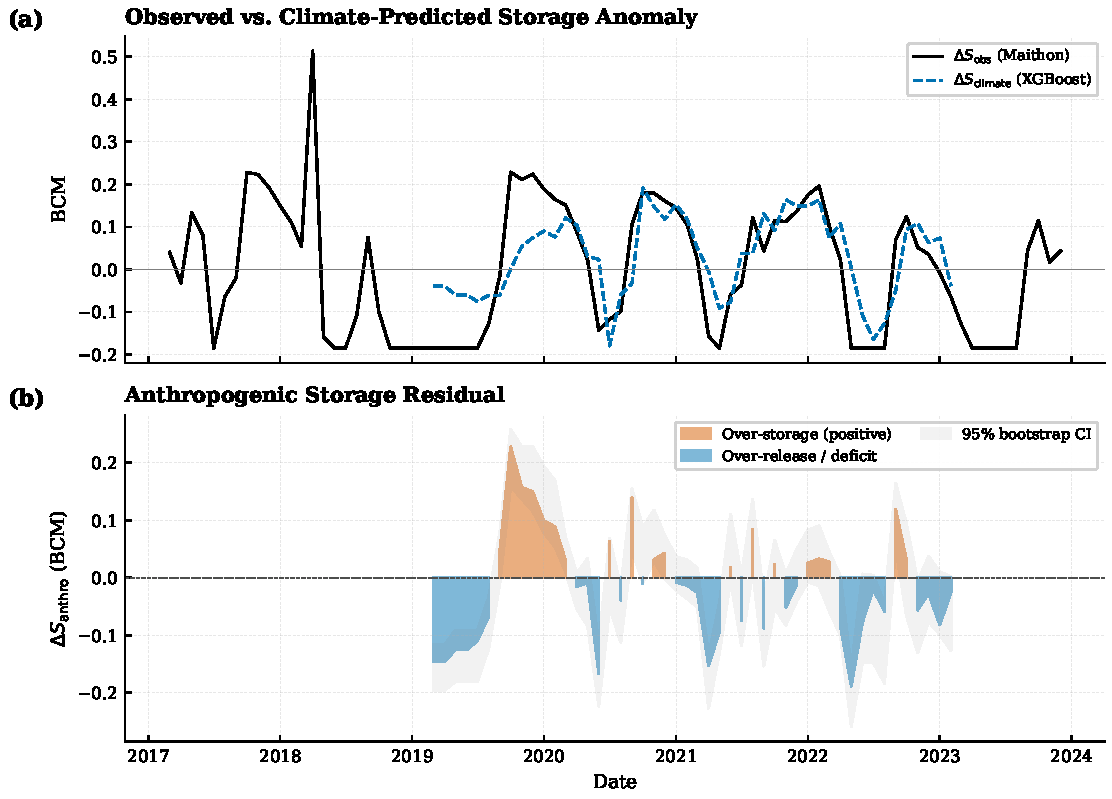
\includegraphics[width=\linewidth]{figures/Fig9_anthro_timeseries}
      \vspace{2pt}
      {\footnotesize\color{gray}
       $\Delta S_{\rm anthro}$ with 90\,\% bootstrap CI.}
    \end{column}
    \begin{column}{0.47\textwidth}
      \small
      Both GRACE TWS and reservoir storage share the
      monsoon annual cycle. A significant $\beta_2$
      could simply reflect that shared seasonality.

      \smallskip
      STL decomposition (robust, period = 12)
      applied to both sides. Regression on
      remainder components only.

      \smallskip
      \begin{exampleblock}{\small Deseasonalised result}
        \footnotesize
        $\beta_2 = +3.41$\,cm/BCM\\
        $p = 0.0003$ (HAC-corrected)\\
        Partial $R^2 = 0.201$
      \end{exampleblock}

      \smallskip
      {\footnotesize Shared monsoon seasonality does not
      explain the result. The signal persists.}
    \end{column}
  \end{columns}
\end{frame}


\begin{frame}{Backup: AV Curve Sensitivity}
  \begin{columns}[T]
    \begin{column}{0.50\textwidth}
      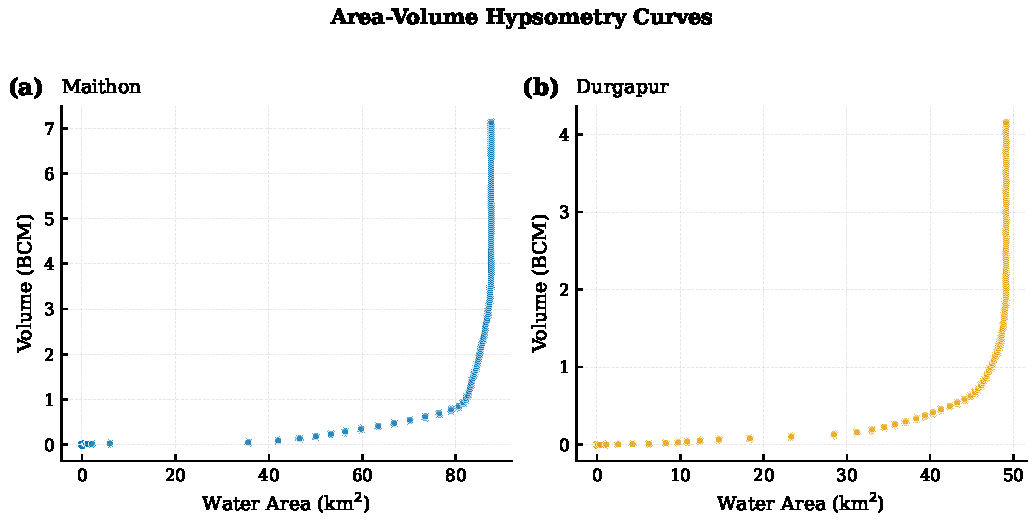
\includegraphics[width=\linewidth]{figures/FigS1_AV_curves}
      \vspace{2pt}
      {\footnotesize\color{gray}
       Area--volume power-law fits for all reservoirs.}
    \end{column}
    \begin{column}{0.47\textwidth}
      \small
      CartoDEM vertical RMSE $\pm$3--5\,m
      in Jharkhand terrain.

      \smallskip
      {\footnotesize
      \begin{tabular}{@{}L{1.4cm}cr@{}}
        \toprule
        Reservoir & $b$ & $R^2$ \\
        \midrule
        Maithon   & 3.0 & 0.97 \\
        Durgapur  & linear & 0.94 \\
        \bottomrule
      \end{tabular}}

      \smallskip
      \begin{block}{\small Perturbation test}
        \footnotesize
        $\pm$10\,\% change to $a$ and $b$:
        $\Delta S_{\rm anthro}$ magnitude shifts
        by less than 8\,\%.

        \smallskip
        Mean sign (negative, indicating net
        managed drawdown) is robust across all
        perturbation scenarios.
      \end{block}
    \end{column}
  \end{columns}
\end{frame}


\begin{frame}{Backup: VIF Filtering Process}
  \footnotesize
  Multicollinearity distorts SHAP attributions.
  Iterative VIF filtering with threshold = 10.

  \smallskip
  {\scriptsize
  \begin{tabular}{@{}L{2.2cm}rL{5.0cm}@{}}
    \toprule
    \textbf{Feature dropped} & \textbf{VIF} & \textbf{Reason} \\
    \midrule
    LC$_{\rm crop}$   & 1,480 & Near-constant over study period \\
    Ni\~{n}o-3.4      & 1,315 & Correlated with DMI \\
    $P$ (rainfall)    & 690   & Absorbed by API$_6$ \\
    SM$_1$ (shallow)  & 661   & Correlated with SM$_2$, PET \\
    Temperature       & 597   & Drives PET and AET (retained) \\
    SM$_2$ (deep)     & 563   & Correlated with SM$_1$, API$_6$ \\
    NTL (night lights) & 191  & Trend only, low variability \\
    NDVI              & 116   & Correlated with temperature \\
    LC$_{\rm for}$    & 106   & Near-constant \\
    $P_3$ (3-month)   & 55    & Absorbed by API$_6$ \\
    \bottomrule
  \end{tabular}}

  \smallskip
  \begin{block}{\footnotesize 8 retained features}
    \scriptsize
    API$_6$, PET, AET, DMI,
    $\Delta S_{t-1}$, $\Delta S_{t-3}$,
    $Q_{\rm inflow}$, MO$_{\rm anom}$
  \end{block}
\end{frame}


\end{document}
